\documentclass[11pt]{report}

\usepackage{setspace}
\doublespacing

\usepackage{tikz}
\usetikzlibrary{positioning, fit, matrix, calc, shapes.multipart, chains, arrows}

\usepackage{syntax}

\usepackage{listings}

% For marking up drafts
\usepackage[normalem]{ulem}

\begin{document}
\title{report}
\author{Tom Hutchings}

\maketitle

\begin{abstract}
  This report covers the design and implementation of an Operating System for the x86 processor platform. It will first give an overview of the broad concept of an Operating System and the tools and technologies that the Operating System will rely on. Then it will discuss a history of the Lisp programming language family in OSs, and how  It will then give the design of a minimal Operating System tailored to provide means to host a high level Programming Language. This language is a custom dialect of Lisp, and is described in the design section along with an interpreter for that language.
  Then the paper will describe an implementation of the OS and Language detailed in the design section, with extracts to demonstrate implementation specific details. Finally the paper will discuss the im TODO
  
\end{abstract}

\tableofcontents
\newpage

\chapter{Introduction}
At the core of almost every running computer exists an Operating System, the software which interfaces between running programs and the computer hardware. The primary purpose of an Operating System is to provide a platform for other computer programs to run on top of, by abstracting away hardware specific details such as memory management and Input and Output to physical hardware.

This paper aims to investigate an approach to Operating System design whereby a high level language is executed by a minimal core OS, allowing the OS to be extended using that language. This ``hosted language'' would be interpreted at run time, rather than compiled ahead of time. Most contemporary Operating Systems are written in compiled languages, requiring restarting the computer they are running on to load any changes to the system. [CITE] By designing an Operating System which hosts an interpreted language, and can be extended in that language, we can evaluate the feasibility of runtime inspection and modification of Operating System code.

\section{Aims}
\begin{itemize}
\item Describe the features and functions of an Operating System;
\item Provide the design for a minimal Operating System, fulfilling the criteria established previously;
\item Establish a design for a high level programming language, and the minimum interface needed for the language to sufficiently extend the OS functionality;
\item Detail the implementation of the proposed OS and Programming Language.
\end{itemize}

\section{Chapter Overview}
\begin{enumerate}
\item Chapter 2: Background will examine the relevant existing material to the development of an Operating System, including CPU architectures and programming languages. Then it will look at use of a high level language in OS development, as relevant to our hosted language.
\item Chapter 3: Design will provide a design for an OS, covering the main design and justifying key design decisions.
\item Chapter 4: Implementation will describe key parts of an implementation of the OS designed, highlighting areas of interest with code listings.
\item Chapter 5: Testing will demonstrate the implementation, and attempt to demonstrate how the implementation addresses the questions posed in the Introduction.
\item Chapter 6: Conclusion will review the paper, and whether it met the stated Aims.
\end{enumerate}


\chapter{Background}

Operating Systems have existed since the 1950s, [CITE] and so a sizable body of both research and implementations exist today, ranging from general purpose OS's to highly specific embedded real time OS's. First this chapter will evaluate what platform to build the OS upon, specifically the CPU architecture to target and the programming language to implement a kernel and interpreter in.

The next section will look at a history of the Lisp programming language, and its use in Operating Systems and compiled applications through history, as it pertains to the development of the high level hosted language that our operating system will interpret.

\section{Target Platform}
Choosing a CPU Architecture to target was an important step, as the OS will have no levels of software abstractions to build upon, itself providing the lowest level of interface to platform specific functionality. Because of this, even when using a compiler which can target multiple CPU architectures, a not insignificant amount of OS code would not be easily portable to other CPU architectures, as the logic of the program itself is architecture specific.

A programming language in which to implement the kernel also had to be chosen. The language must be capable of running in a free-standing environment, i.e. the produced machine code must not link to any external libraries, and must not use any OS facilities such as memory allocation.

To ease development it would be beneficial for the language should to provide an easy mechanism for calling object code generated from external assembly language, as well as allowing for writing of assembly code inline in the language. The language must have a system for directly accessing specific memory locations, e.g. using an absolute address. These are necessary depending on chosen architecture, as some architectures such as Intel's x86 family require initialization to be performed using special assembly instructions which would not normally be emitted by a compiler [CITE: Intel sdm], and certain functions like accessing external hardware can only be used via assembly instructions. The architecture also requires certain data structures to be placed at specific points in memory for initialization, or specific areas of memory must be accessed directly to interface with external hardware.

\subsection{x86}
Intel's x86 family of processor architectures originates in the 8086 CPU, first released in 1978\cite{intel-hall-of-fame}. Over time successive releases built on the iteration, maintaining a degree of backwards compatibility[CITE] but implementing a superset of the previous architecture and adding new extensions to the instruction set. Features such as hardware based Floating Point arithmetic, Single Instruction Multiple Data instructions allowing for parallel data operations, and support for hardware virtualization have been added. This backwards compatible but incrementally improved development model has led to x86 being the primary architecture for personal desktop computers, being the only architecture targeted by all three of the most widely used consumer operating systems, Microsoft's Windows, Apple's macOS, and the free software GNU/Linux OS[CITE].

x86 provides facilities to assist an OS by providing hardware systems to manage memory and access control such as segmentation, paging, and ring levels. Segmentation and paging are memory management and protection schemes, supported on the CPU by a Memory Management Unit (MMU), which helps manage memory via hardware, increasing speed and reducing the OS workload. Memory can be assigned \textit{ring levels} from zero to three, a privilege level which allows a structured system of permissions to be enforced. In most cases only levels zero and three are used, with zero reserved for the OS Kernel and level three provided for user programs, thus separating the privileged kernel from the securely isolated user programs [CITE ring level usage].

\subsubsection{Bootloader}
Upon being powered up an x86 CPU will be in a operating mode called Real-address mode, abbreviated simply to Real mode, a legacy mode with limited memory access. The CPU usually operates in protected mode, and must be switched into this mode. Systems like Segmentation, Interrupts, and Paging are disabled in real mode, and require configuration to be used. [CITE intel sdm 1.3.1].

As the OS will be stored on a storage medium, it must be copied from the medium into working memory. Then the CPU must jump to the loaded OS code and begin execution there. This process of CPU initialisation and OS loading is referred to as Bootloading, and the program that performs this process a \textit{Bootloader}. As these steps are necessary for booting any OS, a common bootloader standard can be devised with which OSs can comply with, and bootloaders could implement. This is the goal of the \textit{Multiboot} specification[CITE multiboot doc], and is implemented by the GRUB2 bootloader[CITE].

Complying with the multiboot specification requires a header to be placed within the first 8192 bytes of the OS image[CITE multiboot doc]. This header exists not only to inform the bootloader that the image is a multiboot compatible OS image, but also to configure certain properties of the bootloader. The bootloader identifies the header by way of a ``magic'' binary value, inserted into the start of the header. As part of the multiboot specification the CPU must be configured to certain requirements after loading the OS. This includes certain register states, configuring the CPU to run in protected operation mode, and placing a structure in memory containing system information which the bootloader has gathered for the OS to use without having to query for itself.

\subsection{C}
C is an imperative programming language, designed from the start for developing Operating Systems, as it was originally developed for the purpose of re-writing the Unix operating system. [CITE] C provides ``low level'' programming features such as direct access to memory locations via the use of pointers, something which many languages abstract away for safety reasons [CITE]. When using the GNU Compiler Collection's (GCC) C compiler, Assembly code for the target CPU Architecture can be written inline with C code, without the need for linking separate files. Finally, C will manage the allocation and deallocation of locally scoped variables automatically, but also allow the programmer to manually manage where variables are allocated in memory, via the aforementioned pointer system. This would allow a kernel written in C to implement a memory allocation scheme which could be utilized both by other OS code and user programs.

As C was first developed around 1972 [CITE], it has numerous compiler implementations, with many different CPU architectures targeted, and many implementations targeting multiple architectures. As of 2020, the GNU Compiler Collection supports emitting compiled code for fifty one architectures [CITE https://gcc.gnu.org/backends.HTML], all of which can be targeted by the GCC C compiler.

\section{Lisp}
Lisp is a programming language family first described as a single programming language in a 1960 paper authored by John McCarthy, principally designed to operate on linked lists. Source code is written in a textual representation of a linked list called an S-Expression, which when evaluated into list form can be manipulated at run time or compile time as a data structure via the use of \textit{macros}[CITE macro stuff].

Implementations with varying execution strategies exist, including Ahead of Time compilation to native machine code [CITE SBCL], using an interpreter [CITE lisp interpreters], and Just in Time native compilation [CITE list jitter]. Since the original language emerged, many new dialects have been developed [CITE], leading to Lisp often being referred to as a language \textit{Family}, rather than a language in and of itself [CITE lisp family].

Common to all these dialects is the S-Expression based syntax, and the ability to manipulate syntax as a data structure, a property called Homoiconicity [CITE homoiconicity]. This allows for the ``programs that write other programs'' paradigm that is commonly used in Lisp programming[CITE lisp metaprogramming], where Lisp \textit{macro} functions generate Lisp code, in the form of linked lists, which is then itself executed.

Lisp pioneered garbage collection[CITE lisp gc], a technique to automatically keep track of allocated objects, and deallocate them when they are no longer usable in the program. This type of automatic memory management lacks the fine grained control over allocation that manual memory management allows, but removes the impetus from the programmer to handle such tasks.

Although Lisp can be either ahead-of-time compiled or interpreted at runtime, development in Lisp is often characterized by an interactive method[CITE lisp interactive dev], where rather than an entire program being compiled and executed, indvidual functions are redefined and altered in the running program, without needing to stop the program and re-compile.

\subsection{Lisp Machines}
Lisp machines are computers specifically designed to execute a Lisp programming language by using hardwarep optimized specifically for the task. These machines were developed during the 1970s due to inadequacies in memory capacity and processing speed of the then current computer systems for running Lisp\cite{knight-lisp}. The solution was to design a computer which was designed from the start specifically for execution of Lisp, with an instruction set that facilitated optimized execution of compiled Lisp code. 

TODO: OS was in lisp


\subsection{Common Lisp}
ANSI Common Lisp is a programming langauge standard devised to unify the variety of Lisp programming languages with a new standard taking elements from each[CITE cl hyperspec]. 

The Common Lisp standard specifies an inteface for compilation of Lisp functions and files. The standard only defines a compiler as ``[a] utility that translates code into an implementation-dependent form that might be represented or executed efficiently'' [CITE http://www.lispworks.com/documentation/HyperSpec/Body/03_ba.htm], leaving the details of the compilation to individual implementations. We can look at how implementations approach compilation and performance on architectures such as x86 to gain insight on how a Lisp system can be optimized for non Lisp machine architectures.

One such implementation of Common Lisp is Steel Bank Common Lisp, or SBCL, takes the approach of a fully compiled implementation [CITE http://www.sbcl.org/manual/index.html], where all code is compiled before being executed. SBCL descends from Carnegie Mellon University Common Lisp (CMUCL)[CITE sbcl docs], itelf a Common Lisp compiler capable of matching C in execution speed\cite{verna2006make}.

SBCL can output compiled object code for a variety of architectures, including x86. 
TODO: what optimisations does SBCL perform

\chapter{Design}
This chapter will describe the design of an Operating System's Kernel and Lisp interpreter in two sections. The design will avoid implementation specific details, instead providing a rigorous but general description of the system. In some cases the design will propose mutliple systems which could be used alternative to each other, any of which the implementation could choose to implement.

The first section will give a design overview of the Kernel, the core of an OS providing an interface with hardware, memory management, and a standard library of utility functions including an interface to request memory allocation and instruct the kernel to free memory regions.

The next section describes a Lisp family language called SYSLISP, it's syntax and built in functionality. It will then give a design for an interpreter of SYSLISP, and the systems required to evaluate and execute the language. Finally it will cover the functionality needed to allow the language to interact with the CPU and memory directly, so as to extend the Operating System by implementing components in its own language.

\tikzset{
  cell/.style={
    rectangle, thick, draw,
  }
}
\begin{figure}[h]
  \centering
  \begin{tikzpicture}
    [node distance = .8cm,
    squarednode/.style={rectangle, draw=black, very thick, minimum size=5cm},]

    \matrix[
    matrix of nodes, nodes in empty cells,
    minimum width = 2cm,
    column sep = 4pt,
    row sep = 10pt,
    text height = 2ex, text depth = .25ex,
    minimum height = 4ex]
    (m) {
      | [cell] | Process & | [cell] | Process & | [cell] | Process & \\
      & & & \\
      & & & \\
      & & & \\
      & & & \\
    } ;

    \node[cell, fit=(m-1-1)(m-1-3), label=center: ]{};
    \node[cell, fit=(m-2-1)(m-2-3), label=center: Userspace]{};
    \node[cell, fit=(m-3-1)(m-4-3), label=center: SYSLISP Interpreter]{};
    \node[cell, fit=(m-5-1)(m-5-3), label=center: Kernel]{};
  \end{tikzpicture}
  \caption{System Architecture}
  \label{sysarch}
\end{figure}

\section{Kernel}
The Kernel's role within the Operating System is acting as the interface between software and hardware. It must manage memory and I/O. The primary tasks for this OS's kernel are initializing the CPU into protected mode, and providing a memory allocation and management system for other code. These are the minimum requirements to allow the hosted language interpreter to run, which can then take over the rest of OS functionality in hosted code.

\subsection{Memory Allocation}
The memory allocator maintains two sequential areas of memory. The first is the \textit{Bitmap}, used to mark which areas of the second, the \textit{Arena}, are in use. The allocator uses a fixed size factor $F$ to map a single binary bit in the Bitmap to a region in the Arena of size $F$. We use a factor $F = 8$, effectively mapping a single bit in the bitmap to an eight bit byte in the arena. On x86 all addressing is byte aligned [CITE sdm], meaning that a factor of eight is the minimum value to ensure byte alignment, and that factor sizes must follow $F = 2^n$ where $n > 3 $.

The allocation process uses a \textit{first fit} method, seeking through the bitmap until it can find a free region large enough to accommodate the size requested. More formally: for an allocation request of size $r$ bits and factor $F$, the allocator must find a contiguous region of $b$ free blocks where $b \geq \frac{r}{F}$.

Freeing a region involves performing the reverse steps, by finding the position in the bitmap to mark as free by taking the address to be freed and dividing it by the factor value, returning the index in the bitmap to be freed. Just like allocation, freeing requires a size argument, for which every bit from the found index to index plus the size is freed. E.g. for address $a = 0x1000$, size $s = 4$ bytes, and factor $F = 8$, we can mark every bit from index $\frac{a}{F}$ to $\frac{a + s}{F}$ as free.

\subsection{Segmentation}
One memory management system that x86 provides is segmentation, a system which allows regions of memory to be divided into segments with different access permissions [CITE intel sdm]. Access rights can be set to mark a segment as Executable or Non-Executable, for example to distinguish a segment containing executable code and a segment containing data. Segments can also be marked with different read and write permissions, forbidding them to be modified, such as in a code segment which shouldn't be altered at runtime.

x86 manages these segments using a data structure called the \textit{Global Descriptor Table}, an in-memory table containing entries which inform the CPU about the segmentation model. Each entry is called a segment descriptor [CITE SDM] and contains four fields: the base address of the segment, the limit, or size of the segment, and the access and flag fields, within which individual bits must be set to enable and disable certain properties of the segment. These include the privilege level of the segment, i.e. what x86 ring levels can access it, whether it can be written to, and whether it can be executed as code or contains non-executable data.

\subsubsection{Flat Model}
A kernel can use a \textit{Flat Model} of segmentation. This configuration essentially provides no memory protection through segmentation, used in configurations where Paging is used for memory protection. Unlike paging, segmentation cannot be disabled [CITE intel sdm], and so a GDT must be configured to satisfy the minimum requirements to configure segmentation correctly, but not enforce any memory protection rules.

In order to do this, four standard segment descriptors must be made in the GDT, one pair for each of the ring levels that the OS will use, in this case ring level zero and ring level three. Each of the two descriptors in the pair have a base value of zero, and a limit value of \textit{0xFFFFF} hexadecimal, and differ only in that one is marked as an executable segment and the other as a writeable data only segment. This effectively removes any restrictions the segmentation system would place on memory sections, as the entire working region of memory is permitted to have any operation performed on it, with any access permissions.

\subsection{Paging}
TODO: x86 paging system \\
how we can implement this with C structs and linked lists \\

\subsection{Interrupts}
Due to the nature of external hardware, events may happen while the OS is not in a position to handle them, or more accurately is not actively polling for an event. A system is needed that allows the hardware to signal that an event has occurred, be handled by the OS, and not alter the state of the CPU. x86 solves this problem using \textit{interrupts}.

The interrupt system of x86 allows for the CPUs program execution to be interrupted, and a new path of execution started, then the original execution resumed when finished.
This allows for the main OS code to run as normal, and when an external hardware event or error occurs the CPU will preempt the kernel, look up the correct interrupt handler function and calling it, whatever caused the interrupt can be handled, and then when finished the CPU can return to what is was doing before the interrupt occurred.

There are three key components to the x86 interrupt system, all of which must be handled by the kernel to use interrupts.

\subsubsection{Programmable Interrupt Controller}
The programmable interrupt controller (PIC) is a hardware device which manages the delivery of interrupts to the processor core [CITE intel sdm 3.10.0]. It receives interrupts from around the CPU and any number of external PICs which handle input and output, then signal that an interrupt has occurred and the IRQ number of the interrupt. The PIC can also receive messages via the system bus, for configuration such as PIC initialization and masking of certain IRQs, and for the processor to send the end of interrupt (EOI) signal to the APIC when it has finished processing an interrupt.

The multiboot standard specifies that the PIC must be left at the values configured by the CPU BIOS [CITE multiboot spec]. Most modern x86 CPUs actually have an Advanced PIC chip, which the CPU BIOS configures to emulate a legacy PIC.

TODO: condense remap and masking (its too much)
These values are configured for a CPU operating in Real address mode, however our kernel will operate in Protected Mode. With these Real address mode settings the IRQ values zero to seven will conflict with the protected mode CPUs exception interrupt values. TODO this bit (remmapping)

As the PIC is a single point at which all interrupt signals must flow through, it's also easy to mask, or disable, certain interrupts from here. Any hardware interrupt from vector zero to two hundred and fifty five can be masked. Masking is achieved by altering the PICs Interrupt Mask Register, 


\subsubsection{Interrupt Descriptor Table}
TODO: IDT is a structure in mem with /gates/ pointing to ISR

The Interrupt Descriptor Table is a data structure stored in memory, similar to the GDT, which contains entries storing the locations of ISRs, or interrupt handlers, in memory. The entries are referred to as \textit{gates}, and their position in the table corresponds to the interrupt vector that they represent.

\subsubsection{Interrupt Service Routines}
function that handles interrupt, returns differently to regular one

An Interrupt Service Routine is a procedure which can be called when an interrupt occurs. There are a few differences between a regular procedure call and an interrupt procedure call which the ISR must account for. The ISR must return using the IRET instruction [CITE sdm], instead of the usual RET instruction. IRET performs additional steps to restore processor state to before the interrupt was triggered, as well as returning from the current point of execution to where it was before the interrupt.
TODO: finish


\section{Hosted Language: SYSLISP}
As the OS is intended not only to host a high level language, but itself be extendable in that language, it was necessary that the OS should manage the parsing and execution. This approach allows for tighter integration between the language and the OS, and could potentially allow for optimization techniques not possible in a user environment. [TODO: cite GC optimization papers from bib]

Considering that any standard library functions must be implemented anew in the OS, access to parsing libraries will be limited due to the effort required to adapt any existing library to use the new OS standard library, instead of the standard library it was written for. This means that parsing of the language must be performed using only the string tools provided to by C, and the new Operating Systems own standard library.

Without the help of tools such as regular expressions and string splitting, we will be limited to individual character comparison, and character string comparison which is trivial to implement from the first. As such, any syntactic complexity in the language would drastically complicate implementation of the parser. [TODO: include example? or cite something about parsing complexity?]

In line with the above requirements, it was decided to implement a dialect of Lisp as the high level language. With a sparse syntax, Lisp is exceptionally easy to parse. Syntactic symbols consist only of three reserved characters and a small, implementation specific set of built-in reserved keywords. [CITE: McCarthy 1960]
TODO: not sure about this line
Lisp is also dynamically typed and garbage collected, as opposed to the static typing and manual memory management of C [CITE].

\subsection{Syntax}
Being a dialect of Lisp, the Operating Systems hosted level language, referred to as System LISP, SYSLISP or SYSL for short, has a simple syntax. Lisp's strengths lie in operations on Linked List data structures, which is also the format that the language is written in. S-Expressions, a textual representation of a linked list, are used to express source code in Lisp, which is parsed into an in-memory list structure and then executed.

SYSLISP syntax can be expressed in BNF notation as shown in figure \ref{fig:bnf}.

TODO: finish BNF grammar
\begin{figure}[h!]
  \centering
  \begin{grammar}
    <s_expression> ::= <atomic_expression> | <list>
    
    <list> ::= ( <s_expression> )
    \alt ( <list> <s_expression> )
    \alt ( <s_expression> . <s_expression> )
    
    <atomic_expression> ::= <symbol> | <numeric>
    
    <symbol> ::= sumn
    
    <numeric> ::= number_or_sumn
  \end{grammar}
  \caption{A Backus-Naur Form represenation of the SYSLISP grammar}
  \label{fig:bnf}
\end{figure}

Note that the only non-identifier terminals in the SYSLISP grammar are ``('', ``)'', and ``.''. Also advantageous of this grammar is it's simplicity and ease of parsing, as it is able to be parsed using an $LL(1)$ parser [CITE?], TODO: LL1 parser

\newpage

The S-Expression syntax forms a textual representation of a linked list, which 

An S-Expression form \texttt{(A . B)} is referred to as a \textit{Cons Cell}, and consists of a pair of values, or pointers to values in memory. Typically in Lisp the first value is called the \textit{car} of the cell, and the second the \textit{car}. Figure \ref{fig:cons} demonstrates the ``box and line'' notation of diagrams representing cons cells.

\begin{figure}[h]
  \centering
  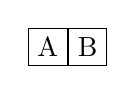
\begin{tikzpicture}[list/.style={rectangle split, rectangle split parts=2,
      draw, rectangle split horizontal}, >=stealth]
    \node[list] (A) {A \nodepart{two} B};
  \end{tikzpicture}
  \caption{A Box and Line notation of a Cons cell with a car of A and a cdr of B}
  \label{fig:cons}
\end{figure}

The pointer can also point to another cons cell. Using this property, we can create a linked list of cons cells by storing a pointer to another cons cell in the cdr of the first cons cell, and the value for each element of the list in the cons cells car. Nested lists can also be created by storing a pointer to a list in the car of a cell.

This linked list which is written as an S-Expression as in figure \ref{fig:conslist}. This syntax can be written in an alternative short hand form, by writing nested cons cells as a single list delimited by parentheses, shown below in figure \ref{fig:conslist}.

\begin{figure}[h]
  \centering
  \texttt{(A . (B . (C . nil)))}
  $=$
  \texttt{(A B C)}
  $=$
  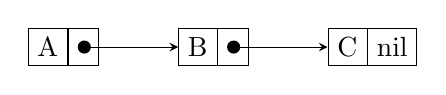
\begin{tikzpicture}[list/.style={rectangle split, rectangle split parts=2,
      draw, rectangle split horizontal}, >=stealth, start chain]

    \node[list,on chain] (A) {A};
    \node[list,on chain] (B) {B};
    \node[list,on chain] (C) {C \nodepart{two} nil};
    \draw[*->] let \p1 = (A.two), \p2 = (A.center) in (\x1,\y2) -- (B);
    \draw[*->] let \p1 = (B.two), \p2 = (B.center) in (\x1,\y2) -- (C);
  \end{tikzpicture}
  \caption{Two equivalent S-Expressions and their cons cell representation.}
  \label{fig:conslist}
\end{figure}

TODO: LL(1) grammar writeup
This syntax facilitates easy expression of lists in text.

\subsection{Interpreter}
One approach to executing a programming language is using an interpreter, a program which parses language input, and directly executes it. An interpreter is able to parse and execute code at runtime, without any ahead of time preparation. This property allows, for example, code to be generated at runtime and executed, or for a user to input code to be executed one expression at a time, have the expression be evaluated and the result of the expression displayed in real time. This is commonly referred to as a Read Evaluate Print Loop, or \textit{``REPL''}. A REPL allows interaction with the program as it is running,  

Lisp interpeters are based around the Eval / Apply dichotomy. These are two functions which can be used together to evaluate any expression in Lisp. As specified in the BNF grammar, a Lisp S-Expression is either a singular \textit{Atomic Expression}, such as a symbol \texttt{x} or numeral type \texttt{52}, or a list written in the form \texttt{(a b c)}, representing a function, e.g. the expression \texttt{(f x y)} is a function application of the function $f$ to the values $x$ and $y$.

These two possible expressions are each evaluated by their respective function, Atomic expressions can be evaluated by \textit{Eval}, and Function applications by \textit{Apply}. When executing a function, each argument is in turn is first \textit{Evaluated} using \textit{Eval}, before being \textit{Applied} to the function using \textit{Apply}. As such function arguments can themselves be expressed as a function application. Consider the expression:

\texttt{(* x (+ y z))}

This Lisp expression represents the mathematical expression $x \times (y + z)$, when written in the infix notation used in mathematics. As arguments are evaluated first, the symbol $x$ is evaluated for it's value as a variable, then the \texttt{(+ y z)} expression will follow the same pattern, where $y$ and $z$ are evaluated as variables, and then applied the $+$ function. The result of that expression is then applied to \textit{(* x)}.

Thus any function expression can be recursively decomposed using the \textit{Eval} and \textit{Apply} pattern. When \textit{Eval} encounters a function expression it will defer to \textit{Apply}. Then, as demonstrated above, \textit{Apply} will defer evaluation of arguments to \textit{Eval}.

TODO: what's a symbol, and how they eval to function and variable

\subsubsection{Environment}
The Lisp interpreter requires a further data structure than just the source program list to execute it. This is the \textit{Environment}, a structure mapping of symbols to values. The environment operates in a heirarchal structure, with each environment containing a reference to a parent environment, until a root environment is reached. This heirarchal structure allows the language to implicitly enforce lexical scoping, by only permitting access to variables defined in the current scope or it's parents.

With the environment in mind, we can view the the Eval and Apply functions as taking two arguments: the source code, and an environment.

When evaluating code symbols can be bound to values, and added to the current environemnt. Then, when evaluating the value of a symbol, the interpreter can follow a recursive procss:

\begin{itemize}
\item Lookup symbol $S$ in current environment. If it exists, return the value and finish.
\item If $S$ does not exist in the current environment then:
  \begin{itemize}
  \item If parent exists, go to parent and repeat process.
  \item If no parent exists, then the symbol does not exist in scope, so we signal an error.
  \end{itemize}
\end{itemize}

TODO: diagram

Some Lisp dialects split functions and variables into separate namespaces. Implementing this system would involve two seperate environment structures [TODO describe env as trees earlier], one for variables and one for functions. Calling a function and accessing a symbols value as a variable use distinct syntax. See fig \ref{fig:funcall}, where the symbol \texttt{f} must be a function as it is being applied to arguments. 

\begin{figure}[hb]
  \centering
  \texttt{(f x y)}
  \caption{Function Call}
  \label{fig:funcall}
\end{figure}

As variables and functions could be syntactically distinguished, in system with seperate function and variable namespaces, the interpreter would be able to unambigously look up the symbol name in the correct environment. In this system functions and variables can share the same name without collision issues, as they reside in different environments.

TOOD: this
The alternative is a single namespace shared by both functions and variables. This system disallows

The environment structure can be implemented in different ways. The only requirement is a system that allows matching keys to values, where keys must be in the form of a Lisp symbol, and values can be any Lisp expression, and for the system to keep a reference to a parent environment structure.

Many Lisp implementations [CITE] use an associative list to implement the structure. An associative list is a list of the form demonstrated as an S-Expression in fig \ref{fig:alist}. This associative list represents a mapping of the symbols {a, b, c} to the values {1, 2, 3}. Other values can be used, such as other symbols, lists, or even Lisp functions. 

\begin{figure}[h]
  \centering
  \texttt{((a . 1) (b . 2) (c . 3))}
  \caption{Associative List S-Expression}
  \label{fig:alist}
\end{figure}

As lookup time for an associative list is $O(n)$, as an environment represented by an associative list grows then the worst case lookup time will grow with it. An alternative implementation to avoid this issue is the use of a simple table or array, which would provide $O(1)$ lookup times, but would either be a fixed size or require a dedicated system to reallocate the table to a larger size when it hits the size limit.

\subsubsection{Label Table}
The Label table is a data structure which allows a symbols label, written as a string, to be replaced with a numeric id. When registering a new label, it will be allocated a slot in the table, represented by the index of that entry within the table. Instead of containing an array of characters, the symbol data structure can just contain the numeric label id. Label comparison operations only require comparing the label id's, rather than comparing each character of the label sequentially.

Looking up the label value in the table is has $O(1)$ complexity, versus $O(n)$ for character array comparison. As the interpreter must look up symbol value at runtime using the label, this effectively moves computation time from symbol evaluation to symbol creation,
TODO: whatever I was doing here

\subsubsection{Standard Functions}
Standard Env functions (defun, let, set, etc) \\
TODO: define form

Alongside the language syntax a set of core built-in forms must be defined. These forms are the building blocks of the language, providing variable and function definition, program flow control, and logical comparison operators. These forms naturally cannot be defined in the SYSLISP language as they make up the language itself, and so must be implemented in the interpreter.

TODO: list basic forms

Further language constructs can be defined in the language itself, by combining these forms to create new forms.
TODO: e.g. greater than equal form definition example

\subsection{Native Interface}
Kernel Env for \\

\chapter{Implementation}
This section will demonstrate an implementation of the designed OS and Language. This implementation is written in C targeting the x86 CPU family. As compiling an OS requires a specialized cross compiler toolchain to be set up, the first part of this chapter will explain the tools used and the process of setting them up.

The next section will describe some key sections of the implementation, with code listings from the implementation used to demonstrate how functionality from the design was implemented.

\section{Toolchain}
GCC, grub-mkrescue, my toolchain build scripts, C/assembly code makefile \\
using macros to allow Lisp interpreter to be run in a normal unix environment for debugging \\

The build system for the OS consists of a cross compiler and a bootloader to build the OS image for booting. A compiler that is shipped as default with most OSs cannot compile an OS, as it requires a specific target architecture to be specified. Instead the approach taken was to build the compiler from the latest source code, configured specifically for the architecture needed.

The compiler used is the GNU C Compiler, targeting \texttt{i686-elf}, Intel 686 family processors and the Executable and Linkable Format standard binary format. In order to ease compilation and updates, a Bash script was written to allow for automated builds. This script installs any system requirements needed to build the compiler via the system package manager, then downloads the a source code tar and performs the steps to build the compiler. Additionally the GNU binutils software, a collection of utilities for working with binary executable files, has to be built. The script also automates this, in a similar process to the cross compiler.

% Is it too large?
%\lstinputlisting[language=bash, caption=The build-gcc.sh script., basicstyle=\tiny]{../toolchain/build-gcc.sh}  

Next is the bootloader. As GRUB2 is being used as our OSs bootloader, we must use the GRUB2 tools on our host computer so they can generate a bootable image from the OS binary. At the time of writing, no are-built binaries for GRUB2 existed on macOS, so the tools had to be compiled from scratch. As with the compiler, a build script was written to automate the process.

Finally, with the build tools ready, the OS can be built. The implementation uses the GNU Make software to manage builds, where a configuration file called \texttt{Makefile} specifies how to perform the build.

\lstinputlisting[language=make, caption=Makefile, basicstyle=\small]{../os/Makefile}

\section{Kernel}
\subsection{Booting}
boot.S and multiboot header \\
kernel init \\
lisp entry \\

\subsection{Memory Management}
memory allocator \\
gdt code extracts \\

\subsection{Interrupts}
PIC and IDT extracts \\
calling between assembly and C, Interrupt call system and stack state \\
OS interrupt registration system (and how it differs from simple IDT gates) \\

\section{Language}
\subsection{Parser}
C implementation extracts \\

\subsection{Interpreter}
Eval/Apply implementation listings \\
symbol table implementation \\
Lisp Environment implementation (is in C struct rather than usual Lisp alist) \\
nativef1-5 vs lispf calling types \\

\subsection{OS Integration}
show Kernel Env src and how it allows memory access and inb/outb calls \\
datatype conversion, u8, u16, and u32 vs num type and ensuring memory access type safety \\
ptr pointer type \\


\chapter{Testing/Evaluation}

\chapter{Conclusion}
\section{Future Work}


\bibliographystyle{ieeetr}
\bibliography{bib/report}

\end{document}